	\addtocontents{lof}{\protect\addvspace{10pt}}
	\addtocontents{lof}{\protect\contentsline{figure}{\textbf{Full Size Figures}}{}{}}
	
	
	\section{Full Size Images}
	\begin{figure}[H]
		\centering
		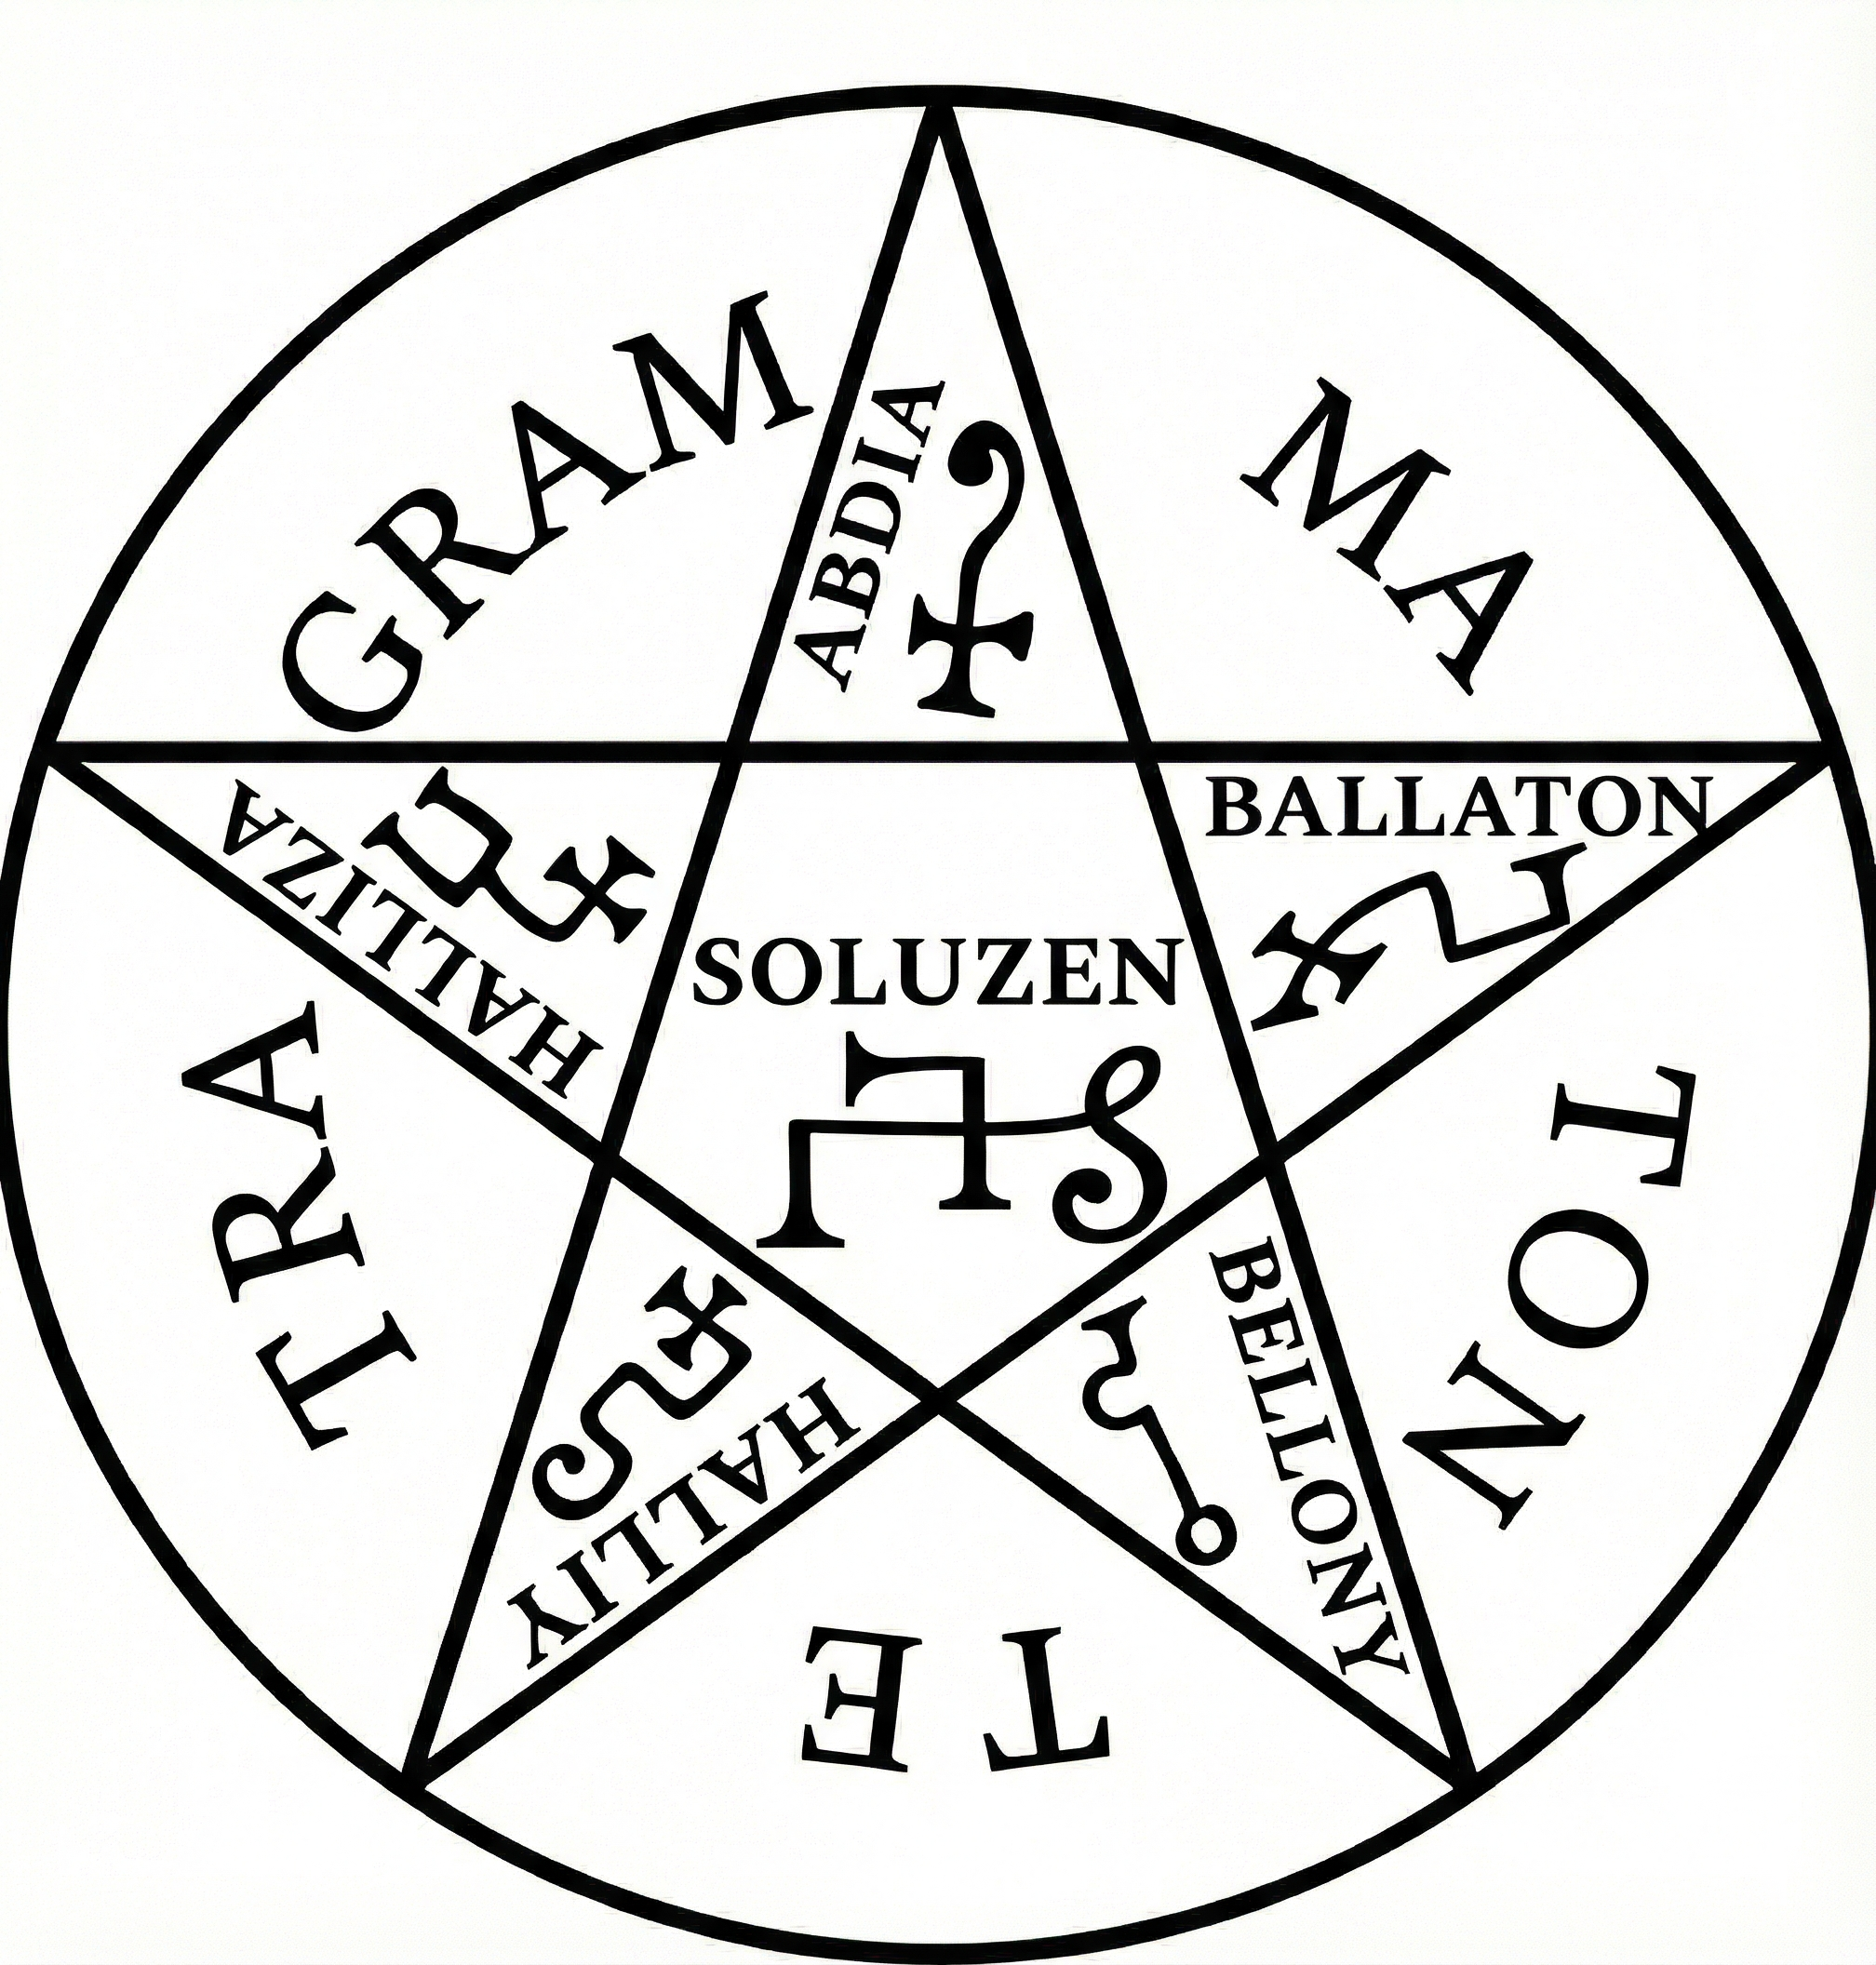
\includegraphics[width=0.8\textwidth,height=0.8\textheight,keepaspectratio]{solomon_pentagram.png}
		\caption{The Pentagram of Solomon}
		\label{fig:solomonpentagramfull}
	\end{figure}

	\clearpage
	\begin{figure}[p]
		\centering
		\includegraphics[width=0.8\textwidth,keepaspectratio]{solomon_hexagram.png}
		\caption{The Hexagram of Solomon}
		\label{fig:solomonhexagramfull}
	\end{figure}

	\clearpage
	\begin{figure}[p]
		\centering
		\includegraphics[width=0.8\textwidth,keepaspectratio]{solomon_triangle.png}
		\caption{The Triangle of Art}
		\label{fig:solomontrianglefull}
	\end{figure}

	\clearpage
	\begin{figure}[p]
		\centering
		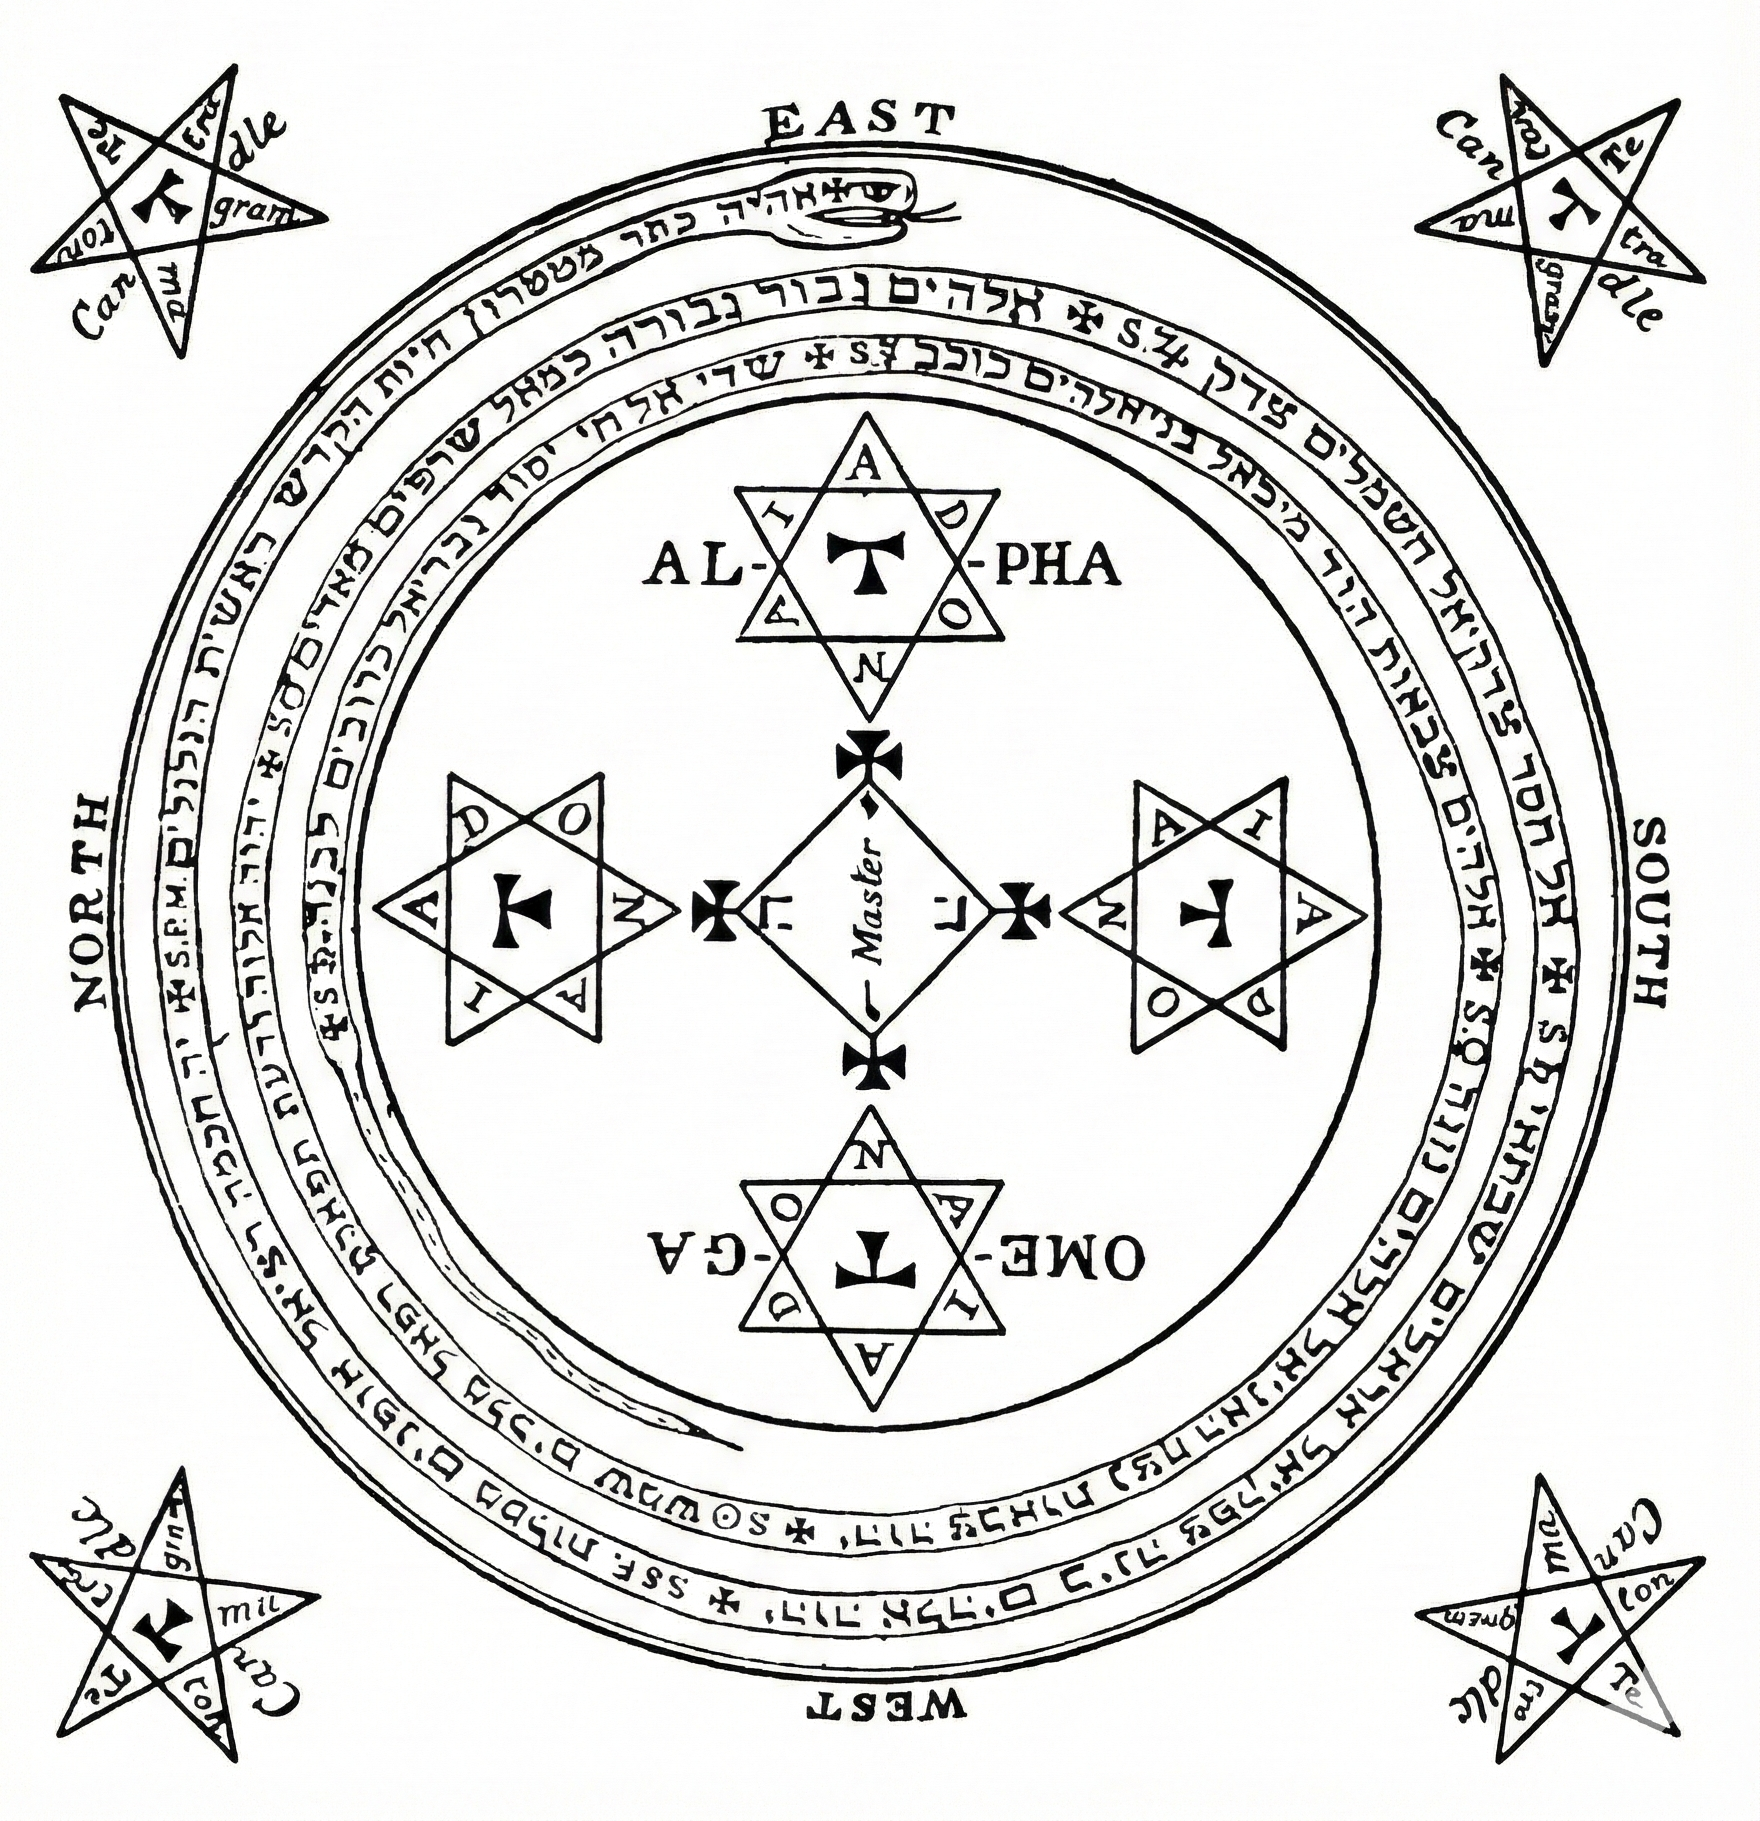
\includegraphics[width=0.8\textwidth,keepaspectratio]{solomon_circle.png}
		\caption{The Circle of Solomon}
		\label{fig:solomoncirclefull}
	\end{figure}

	\clearpage
	\begin{figure}[p]
		\centering
		\includegraphics[width=0.8\textwidth,keepaspectratio]{solomon_circle_and_triangle.png}
		\caption{Circle and Triangle}
		\label{fig:solomonfrontfull}
	\end{figure}

	\clearpage
	\begin{figure}[p]
		\centering
		\includegraphics[width=0.8\textwidth,keepaspectratio]{benedict_face.png}
		\caption{Detail of the Front Inscription (Crux S. Patris Benedicti) \cite{stutler_medal}}
		\label{fig:benedictfrontfull}
	\end{figure}

	\clearpage
	\begin{figure}[p]
		\centering
		\includegraphics[width=0.8\textwidth,keepaspectratio]{benedict_cross.png}
		\caption{Detail of the Reverse Inscription (Crux S. Patris Benedicti) \cite{stutler_medal}}
		\label{fig:benedictcrossfull}
	\end{figure}
	
	\clearpage
	\begin{figure}[p]
		\centering
		\includegraphics[width=0.8\textwidth,keepaspectratio]{st_anthony_brief_shield.png}
		\caption{Saint Anthony's Brief on a Shield}
		\label{fig:st_anthony_brief_full}
	\end{figure}

	\fullsizeimage{st_anthony_brief_cross.jpg}{Cruciform Brief of Saint Anthony}{c. 1880.  Private Collection}{anthony_brief_source}

	\clearpage
	\begin{figure}[p]
		\centering
		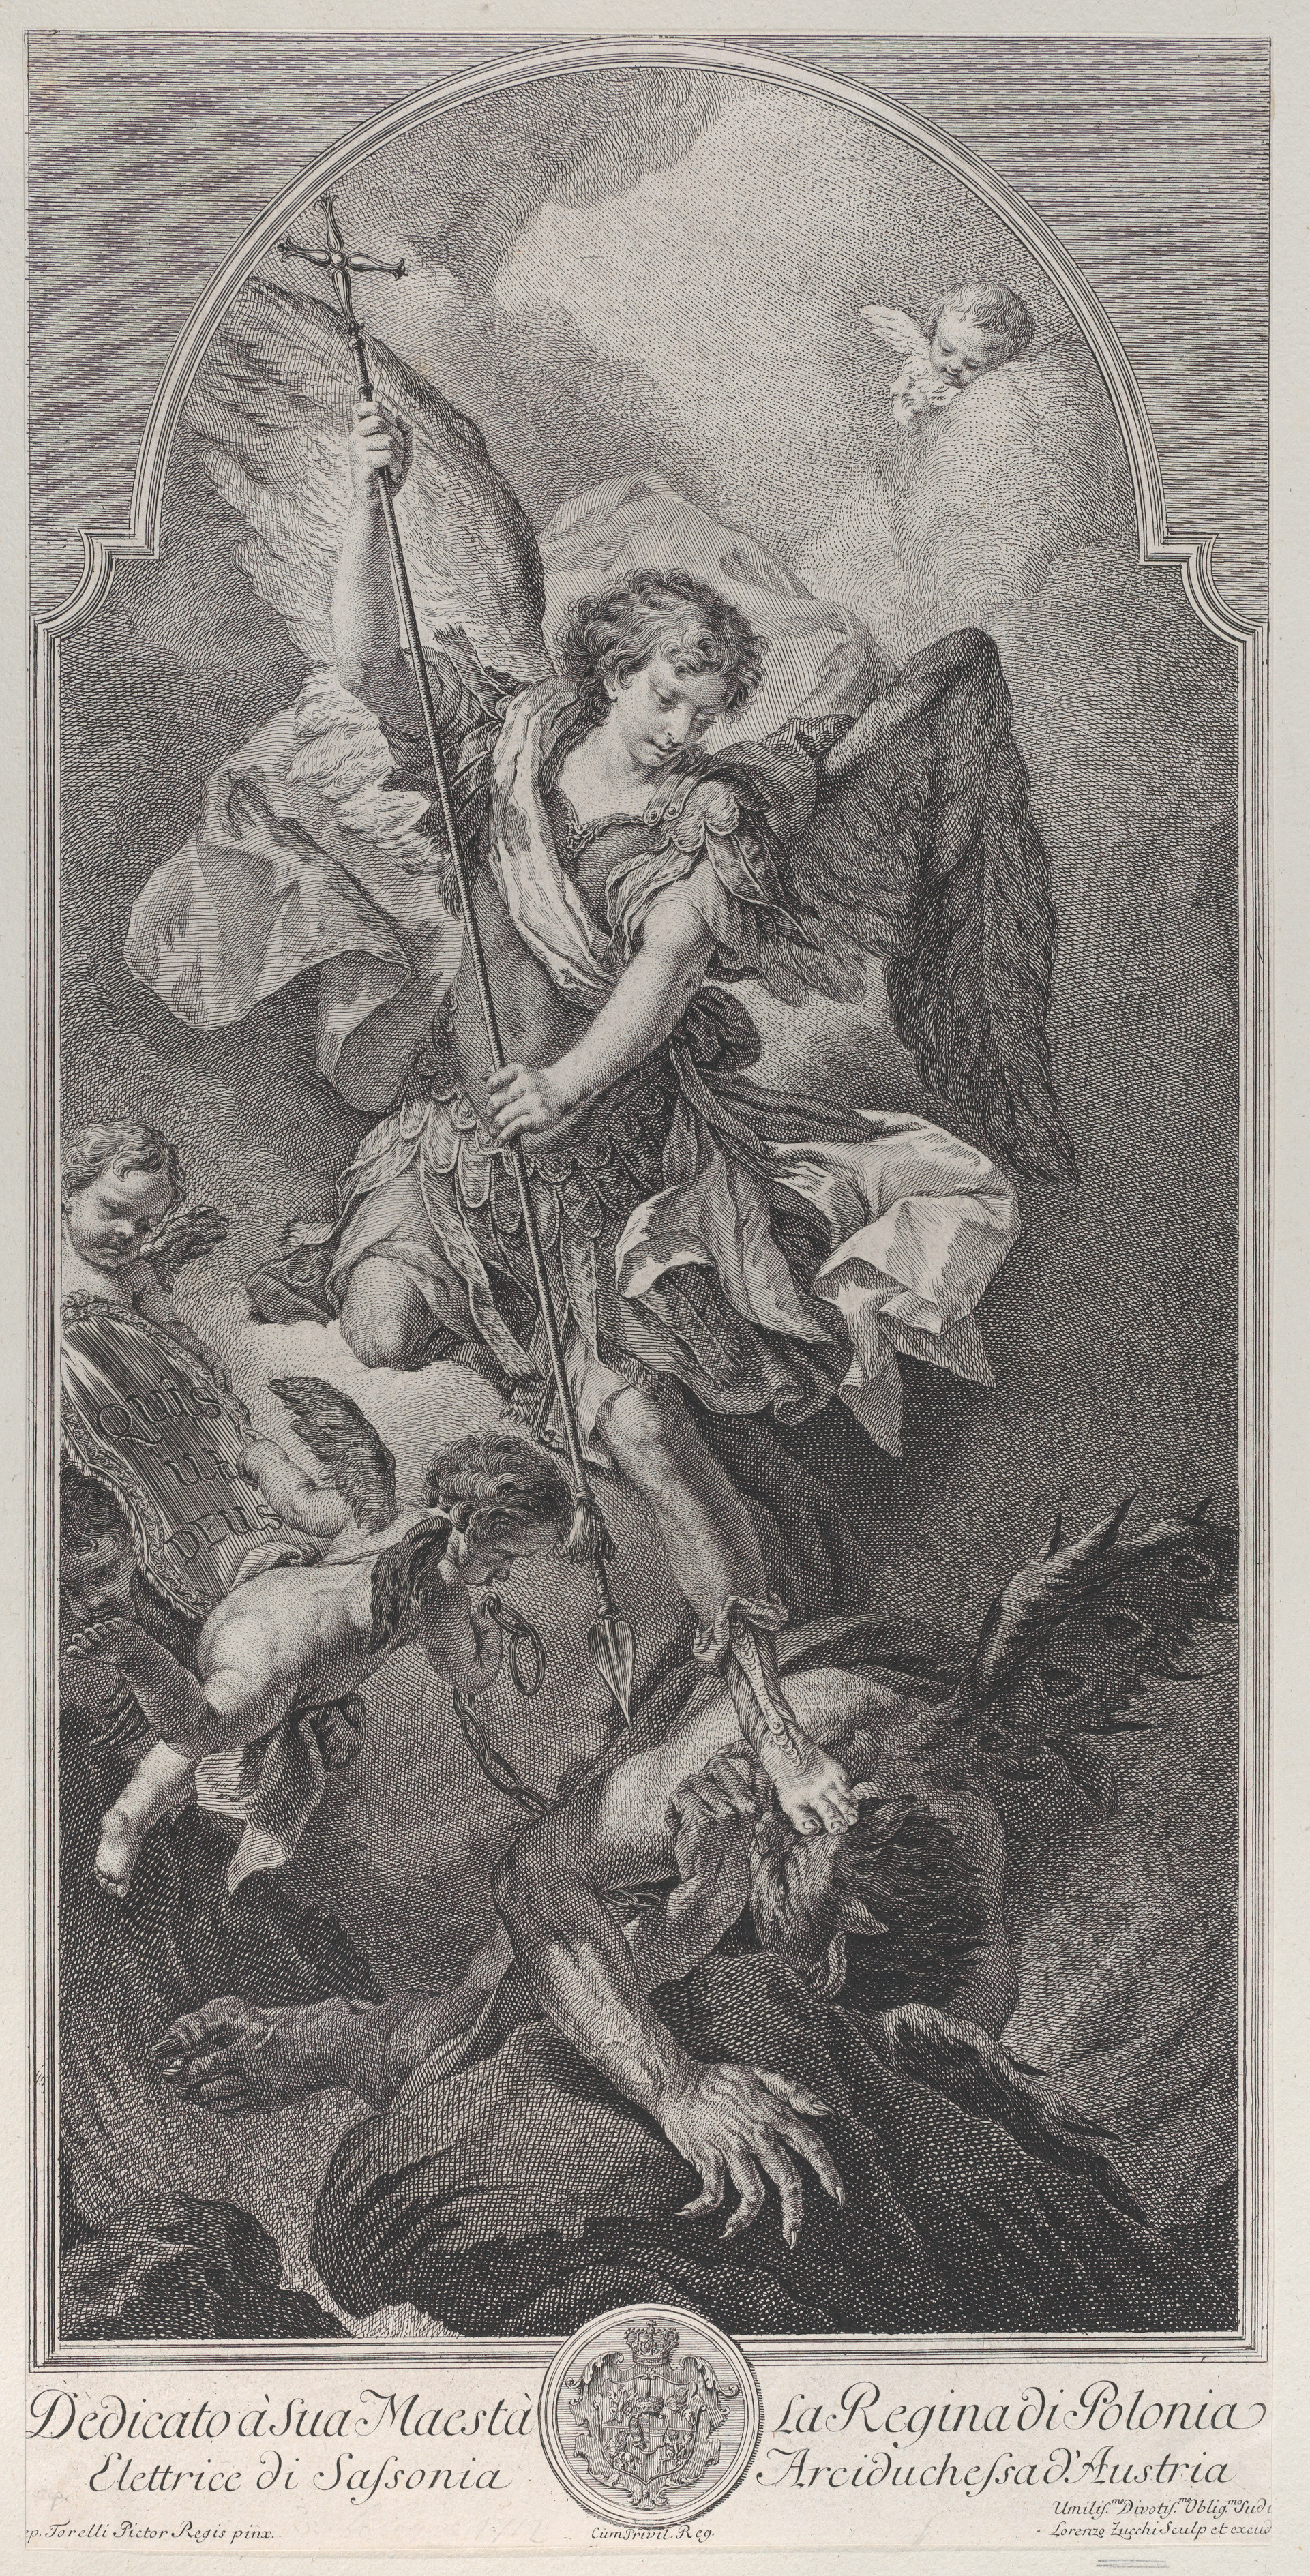
\includegraphics[width=0.9\textwidth,height=0.9\textheight, keepaspectratio]{st_michael_defeating_satan.jpg}

		\caption[St. Michael Detail]{The Archangel Michael defeats Satan.\\
		\textit{Lorenzo Zucchi (Italian, 1725--1779). Engraving after Stefano Torelli.}}

		% \nocite ensures it is still in the bibliography list, even though we didn't use brackets here
		\nocite{met_michael}
		\label{fig:st_michael_full}
	\end{figure}
	
	\fullsizeimage{tobias_woodcut.jpg}{Tobias Catching the Fish}{Ninth German Bible (Anton Koberger, 1483)}{koberger_bible}
	
